\section{Introduction}
Today, learning systems have gained significant attention in the literature for the overwhelming popularity of machine-learning (ML) related workloads. Most of work to date in the systems and architecture community has focused on improving the efficiency of evaluating trained models. This makes sense given that a model is trained only once but can be used many times for inference. However, arriving at a trained model frequently requires experimentation, and thus multiple training runs, each of which may take days. Accelerating the training process lets ML scientists iterate faster and design better model.

Traditionally, training has been viewed as a compute-bound problem, best done in a single large compute node with many accelerators. However, the ever-growing data volume pushes for monster-sized models, a scale even the exponentiation of compute power growth in single device couldn't handle. As ML models get bigger, training time gets prohibitively longer. Timely training requires exploiting parallelism with a distributed system.

\begin{table}
\centering
\begin{tabular}{|c|c|c|c|c|}
  \hline
  Models & Complexity & Size & Time & Configuration \\
  \hline
  Linear Regression~\cite{seber2012linear} & O($D^3+ N^2D$) & Small & Short & CPU \\
  \hline
  SVM~\cite{wang2005support} & O($N^2D^2$) & Small & Short & CPU \\
  \hline
  GBDT~\cite{friedman2001greedy} & O($TLFN$) & Small & Short & A few CPUs \\
  \hline
  \hline 
  AlexNet~\cite{alexnet}   & 0.0058 & 48M & 6 days  & 2x GTX 580\\
  \hline
  ZFNet~\cite{ZFNet}   & 0.0062  &  $\approx$48M  & 12 days  & GTX 580\\
  \hline
  VGGNet~\cite{VGGNet}   & 0.12  & 137M & 15 days & 4x Titan Black\\
  \hline
  GoogleNet~\cite{GoogleNet}   & 0.03  & 9M & 7 days & A few GPUs\\
  \hline
  ResNet~\cite{RESNET}   & 0.117 &  58M & 21 days & 8x GPUs\\
  \hline
  Xception~\cite{Chollet_2017}  & 5.0  & 22M & 30 days & 60x K80\\
  \hline
  \hline
  BERT~\cite{bert}  & 3.8 & 340M & 4 days & 16x TPUs v2 \\
  \hline
  GPT-2~\cite{GPT2}  & 248 & 1.5B & 7+ days~\cite{gpt2Time} & 256x TPUs v3 \\
  \hline
  \hline
%  Device Placement~\cite{mirhoseini2017device} 2017 & - & 27 hours & 80 GPU nodes  \\
%  \hline
  NAS~\cite{zoph2016neural}  & 31 & 86M & 28 days & 800 K40 GPUs\\
  \hline
  AlphaGoZero~\cite{silver2016mastering}  & 1800 & - & 1 day & 5000x TPUs \\
  \hline
\end{tabular}
\caption{A few representative machine learning techniques and models that support increasingly complex tasks (trees, support vector machines, neural networks) and their complexities to train (pfs-day, or days to train computing at 1 PFlop/s. 1PF/s roughly corresponds to 64 Tesla V100 GPUs FP32, or 8 with mixed-precision FP16, running at peak throughput), and their reported training time and the machines they are trained on. We used the same method of estimating complexity as in the original OpenAI blog post~\cite{AIandCom3:online} for the additional models in the table. $D$: features. $N$: samples. $L$: leaves per tree. $T$: number of trees to build.}
\label{table:trend}
\end{table}

Table~\ref{table:trend} gives a taste of the evolution of machines learning models/techniques: they are getting increasingly more demanding in terms of compute resources, such that the use of hundreds or even thousands of machines and accelerators for weeks is commonplace. 




The most common way of exploiting parallelism, ``data'' parallelism, consists of a computation-heavy local computation phase and a communication-heavy parameter exchange phase. Efficient distributed training involves optimizing both stages. Many past work demonstrate the solution of accelerating these processes by building specialized hardware clusters with fast interconnects ~\cite{DBLP:journals/corr/abs-1711-00489, You:2018:ITM:3225058.3225069, DBLP:journals/corr/abs-1711-04325,jia2018highly,DBLP:journals/corr/abs-1811-05233,sun2019optimizing, ImageNetIn1Hour, firecaffe, phubsocc}. While the results are encouraging, as we shall see, faster hardware is not panacea: the unstreamlined software stack and unbalanced compute to communication resource allocation prohibits utilizing full capability of the hardware, and the compute units are more likely than not waiting on the network because the latter simply cannot keep up (Figure~\ref{fig:clusterOverhead}). We expect the problem not going away on its own, because of the observed trend at which the network capability is growing is significantly outpaced by that of the compute resources (Figure~\ref{fig:accthroughput}).  


\begin{figure}
	\centering
	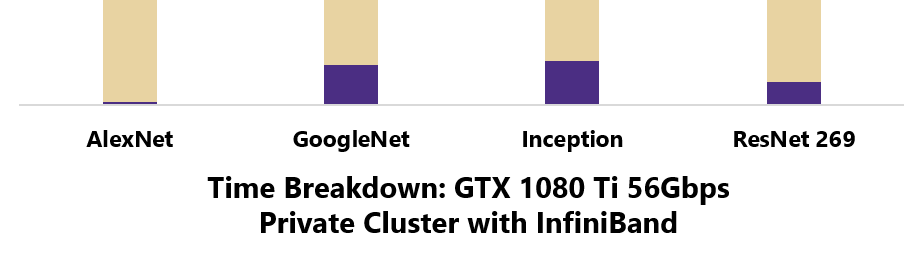
\includegraphics[width=.5\linewidth, trim=6 1 3 3,clip]{Figures/clusteroverhead.png}
	\caption{Even with a fast, small-scale cluster, communication still takes most of the time duration training, wasting compute resources.}
	\label{fig:clusterOverhead}
\end{figure}

\begin{figure}
	\centering
	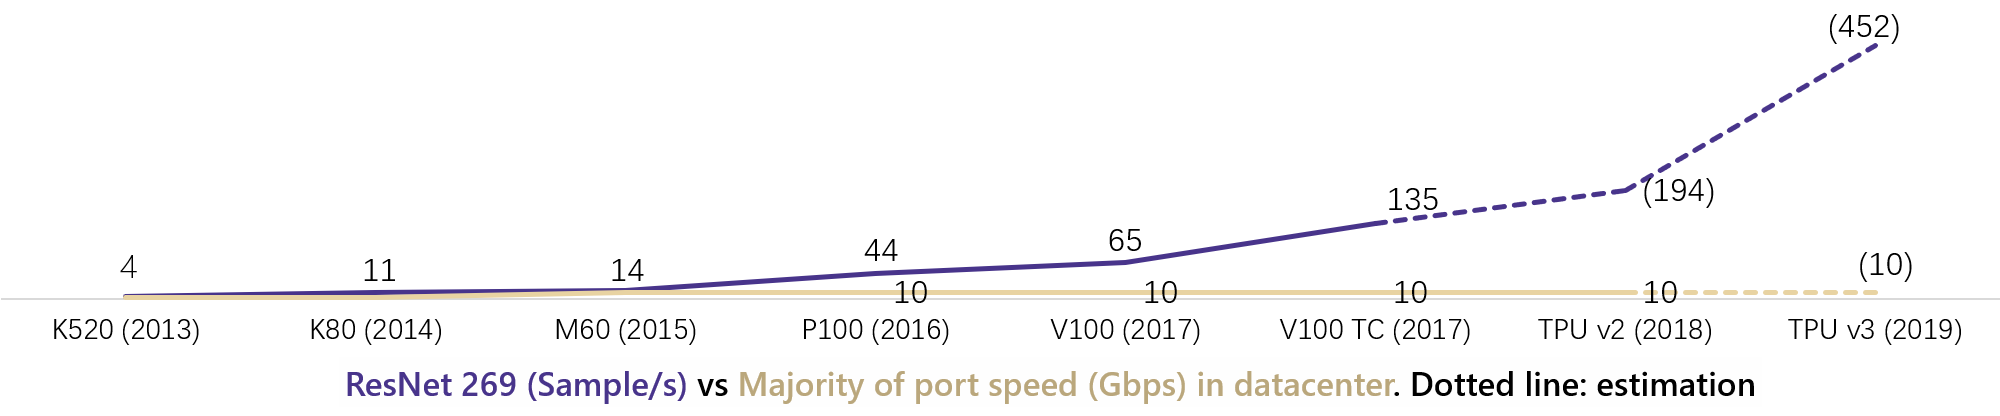
\includegraphics[width=\linewidth, trim=2 3 3 3,clip]{Figures/computevscomm.png}
	\caption{Throughput for an industry standard benchmark (ResNet) has seen an improvement of 35x, and is estimated to increase by 100x with latest accelerators. GPU performance tested with MxNet on EC2. TPU throughput estimated based on TensorCore's measured performance. Estimation for majority of the port speed of datacenters is based on Cisco study~\cite{CISCOMarket}. Only until very recently did the public cloud start offering 100Gbps bandwidth instances on standalone VMs~\cite{Introduc9:online, NewC5nIn6:online}}.
	\label{fig:accthroughput}
\end{figure}

To tackle these problems, a comprehensive codesign of software stack and hardware configuration is required. To that end, we provide a template for speccing an entity called \pbox that provides the near perfect communication to computation balance for acting as a parameter server in a distributed training job, and a companion piece of software, \phub that streamlines handling over gradient  transfer, aggregation and model optimization by carefully extracting locality inside a physical host and latency hiding. 

While \pbox and \phub are effective, it is important to understand accelerating training in these specialized, privately-owned clusters does not complete the story: first, those hardware setups require steep investment and only a few have that luxury; second, since it is much easier to thoroughly optimize the entire stack in private clusters as we have control over the entire system, some optimizations are not always possible to be applied universally.

An alternative to owning a private cluster is renting VMs from the public cloud, which has become a popular, more accessible approach. Currently, all major cloud providers offer racks of nodes with specialized accelerators (such as GPUs, TPUs, and custom FPGAs)~\cite{GoogleCl74:online,MachineL50:online,DeepLear23:online,sagemaker,brainwave,Jouppi:2017:IPA:3079856.3080246,222611} for ML workloads. But at the same time, scalable training in the public cloud isn't just a straightforward application of \pbox and \phub optimizations.

\begin{figure*}[t!]
	\centering
	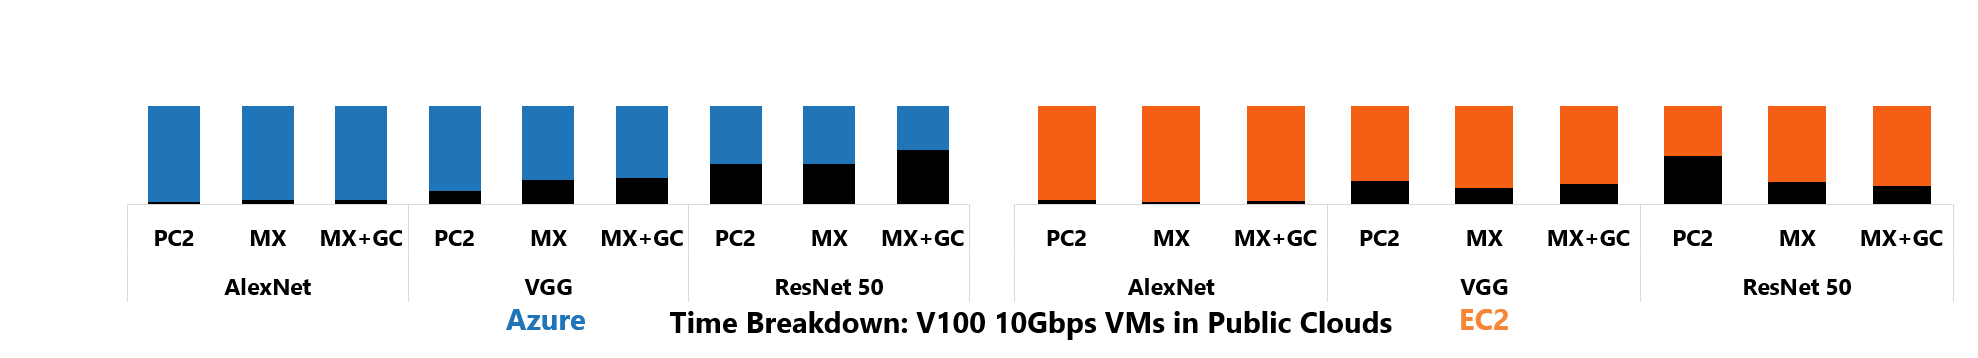
\includegraphics[width=.9\linewidth, trim=6 1 3 3,clip]{Figures/cloudoverhead.png}
	\caption{Even with state of the art training frameworks and recent optimizations, up to 90\% of time during cloud-based training of popular models is wasted explicitly waiting on the network in the public clouds.}
	\label{fig:cloudOverhead}
\end{figure*}


Even with modern frameworks and recent optimizations 
(e.g., gradient compression and quantization~\cite{lin2017deep, cntk1bt, lim20183lc}, latency-hiding~\cite{poseidon, jayarajan2019priority,hashemi2018tictac}, optimized communication libraries~\cite{facebook35:online, Operatio73:online, dmlcpsli50:online} and large batch optimizations~\cite{ImageNetIn1Hour}), distributed training at scale on the public cloud still incurs high overhead: up to 90\% of total training time can be wasted waiting on the network (Figure~\ref{fig:cloudOverhead}). Further, existing solutions so far focus solely on addressing the \textit{bandwidth} bottleneck, and ignores cloud-specific challenges: the hierarchical network structure in datacenter breaks the usual assumption of link speed being uniform; multi-tenancy and the dynamic nature of the cloud traffic cause high variation in performance. All these add to the complexity of scaling up distributed training and can render existing solutions less effective. 

Accelerating cloud-based distributed training thus requires paying attention to a third dimension (apart from software and hardware): the environment. First, we need an aggregation mechanism that is appropriate for network topologies that display bandwidth oversubscription, and that makes appropriate use of underprovisioned links.  Second, we need to be able to identify the underlying network topologies and bandwidth/latency constraints (or collectively, locality) even if the public cloud does not expose such information.  Finally, we need communication schemes that can react to changing network conditions, especially in the presence of interfering traffic generated by other tenants. Our solution is collectively called \plink, an optimized, locality-aware system that uses a fitted hierarchical aggregation scheme to extract locality from the underlying datacenter network, based on end-to-end network probes and dynamic network load.

With \pbox, \phub and \plink, we complete the picture of accelerating machine learning of all kinds, ubiquitously, with efficient implementation of parameter servers. In the following sections, we start with an overview of the mechanism of distributed training, then we walk through each of the proposed solution in detail. We show how specific optimizations adopted target directly at the bottlenecks in each scenario and lead to end-to-end speedup in real-world learning tasks.